\note{Sloppy/Intuitive Reasoning v. Precise Reasoning Using �The MODELS�}{If you run out of time in \DL, this activity can  be finished as an \FNT{}.  Make sure they get through the ``Try It Out'' and its associated \WC{} discussion, so everyone knows the actual behavior.}
\section{Explicit Reasoning Using Models}
\label{act2.2.3}

\begin{overview}

	\textbf{Overview:} Now that we've discussed many different physical scenarios, our models probably have become second nature to you. Maybe so much so that we may have to revisit how to explicitly model a phenomenon. We'll do that with a new phenomenon.

\end{overview}

\note{Make sure each table has the apparatus needed to perform these activities.}{
Groups need to get their predictions made and on the board before trying the activity.  THIS IS IMPORTANT!  The fact that the result is not obvious makes the activity interesting, because there are several ways to argue it when NOT using THE MODEL.  By applying the energy-interaction model, it is possible to understand why the systems behave as they do. 
Make sure the difference in the two masses is the same in set 1 as it is in set 2.  It doesn�t really matter what values the masses are, as long as the difference is the same.  
That being said, you want the difference to be fairly small, so the motion is �slowed down,� but not so small that frictional effects in the pulley become significant.  If the pulley seems to have considerable friction, you will need to tell the students to increase the mass difference.  The system must continually accelerate when released, not come to a constant speed. 
}

\subsection{Two Masses Over a Pulley -- Atwood's Machine}

\begin{benumerate}
	\bitem{Think and Discuss}
	
	Imagine this situation:  A string connecting a smaller mass, $m$, and a larger mass, $M$, passes over a small pulley that is almost frictionless.  The masses are initially held at rest; then are released and allowed to move:
	
	\begin{center}
		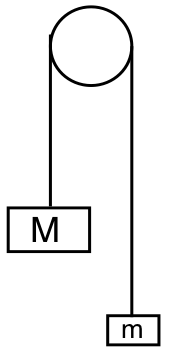
\includegraphics[width=0.1\linewidth]{act223-atwood}
	\end{center}
	
	\note{Predictions and Trying it out}{
Step in and help the groups (two tables working together).  The two groups can release their masses at the same time to more clearly see the difference in final speed.  MAKE SURE STUDENTS SEE CLEARLY WHAT ACTUALLY HAPPENS.

In the \WC{} Discussion, compare some of their intuitive predictions with what actually happens.  Some predictions will be correct, some will not.  EMPHASIZE that now by carefully applying the model we can be absolute sure which should happen and/or can explain why it does happen the way it does.
	}
	Based on your intuition which set of attached masses, each differing by \unit[20]{g}, will move faster when released?
	
	\begin{center}
	\begin{tabular}{lll}
		\textbf{Set A:}	&	$M_A = \unit[220]{g}$,	&	$m_A = \unit[200]{g}$\\
		\textbf{Set B:}	&	$M_B = \unit[70]{g}$,	&	$m_B = \unit[50]{g}$
	\end{tabular}
	\end{center}
	\begin{center}
		\begin{tabular}{ll}
		\textbf{Circle your choice here:}	&	(a) Set A moves faster\\
								&	(b) Set B moves faster\\
								&	(c) Both move with the same speed
	\end{tabular}
	\end{center}	
	
	\bitem{Put your group's choice on the board}
	
	How sure are you about your reason(s) and predictions? What is your intuition based on?
	
	\bitem{Try it out}

	Pair up with an adjacent table.  One table will attach the heavier set of masses, the other table should attach the lighter set. Try it out and see which set moves faster. 
	
	What do you observe?
\WCD
\end{benumerate}

\subsection{Applying the \EnergyInteractionModel{}}
\label{act2.2.3-2}

Apply the \EnergyInteractionModel{} to the two-masses-over-a-pulley situation. Model this system as if the pulley is massless and frictionless, so you won't have to worry about energy systems associated with the pulley.\\

\noindent Take the \textbf{initial state} to be just as you release the masses (what is $v_i$? what is $\Delta v$?).\\

\noindent Take the \textbf{final state} to be when the masses have moved a distance $d$ and have speed $v$, but before they hit anything or run out of string.\footnote{Since $d$ denotes a distance, it is a positive number; so, $\Delta y = \pm d$, as appropriate.}

\note{}{
	Students should identify four energy systems ($PE$ and $KE$ for each mass).  The critical and difficult step for many students is that $KE$ is going up for both but $PE$ is going down only in the large mass.  Make sure they have all arrows drawn correctly for the change in energy for each of the four systems.

	They should have the following expressions of energy conservation as part of their diagram:
	\[\Delta PE_{grav,1}+\Delta PE_{grav,2}+\Delta KE_{1} + \Delta KE_{2}=0\]
	\[\Delta m_{1}g(+d)+m_{2}g(+d)+\frac{1}{2} m_{1} v^{2} +\frac{1}{2} m_{2} v^{2} =0\]
	The assumptions �massless� and �frictionless� mean we are ignoring rotational KE and thermal energy.
}	

\begin{enumerate}
	\item Create a particular model of the phenomenon described above by constructing a complete \EnergyDiagram{} for \textbf{each} of the mass sets using the initial and final states described above.
	\item	\label{act2.2.3-(2)} When you substitute algebraic expressions for changes in individual energy systems in the algebraic representations of your particular \EnergyInteractionModels{}, you will find the symbols $m$, $M$, $g$, $v$, and $d$ useful. Watch your ``minus signs!''
	\item One important practical use of the \EnergyDiagram{} is in the interpretation of algebraic expressing of energy conservation. For example, what do each of the terms in the equation mean, and what should their sign be? Check, and be ready to show, that the signs of the terms in the equation from \eqref{act2.2.3-(2)} are consistent with the increases and decreases in energy of the energy systems in your diagram.
	\item\label{act2.2.3-(4)} What energy systems have you ignored by your assumptions about the pulley?
	
	[You don't have to put \eqref{act2.2.3-(4)} on the board.]

	
\WCD  
\end{enumerate}
 
\subsection{Reasoning and Explaining with Particular Models}
\label{act2.2.3-3}

You have constructed two particular \EnergyInteractionModels{}, one for each of the different sets of masses. You are now going to use these models to make sense of and explain why one set of the masses (the set with the smaller masses) moved faster than the other set.

\todo[inline]{Should the ``\EnergyInteractionModels{}'' here be ``\EnergyDiagrams{}''? The same goes for any uses of the word ``model.''}
\note{Make sure everyone understands the diagrams and equations}{}

\subsubsection*{Comparing the changes in energy of the various energy systems}


  
\note{}{Since the speed of both masses is increasing, the total KE is increasing.}
\begin{enumerate}
	\item During the process (from beginning to end), does the total $KE$ of the two masses (the sum of the $KE$s) increase, decrease, or stay the same? How do you know?  Is your response the same for both the heavier and the lighter pair of masses?
	\label{act2.2.3-(5)}
	
	\note{}{Both systems have a net decrease in PE. }
	\item During the process, does the total $PE$ of both masses (sum of the $PE$s) increase, decrease, or stay the same? How do you know?  Is your response the same for both the heavier and the lighter pair of masses?
	
\note{}{The essential part here is realizing that the sum of the PEs involves the difference in masses, which were set up to be the same in both cases, so the total change in PE for both cases is the same.}
	\item Compare the magnitudes of the total change in $PE$ of both masses that occurs during the process across the two systems (the heavier pair and the lighter pair).  Are the total changes the same or different?  Explain.
	
\note{}{Since the total change in PE is the same for both sets, the total change in KE must also be the same.}
	\item Compare the magnitudes of the total change in $KE$ of both masses that occurs during the process across the two systems (the heavier pair and the lighter pair).  Are the total changes the same or different?  Explain.
	
\note{}{The question has to do with speeds , which is related to change in KE, but KE involves the total mass as well as the final speed.  It is the total mass that differs between the two systems.}
	\item Did the original question regarding the two sets of masses have to do with the $KE$ of the masses or something else?  Was it related to the $KE$?  Compare this across the two systems (the heavy pair and the lighter pair).  Is this the same or different?  Explain.
\note{}{Prompt \ref{act2.2.3-(9)} is the same as \FNT{} \thechapter-\ref{fnt2.3.1-1} on today�s exit handout.  Do not go over it in class.  Emphasize that students need to practice writing an explanation like this in preparation for future quizzes.}

	\label{act2.2.3-(9)}
\end{enumerate}

\subsection{Creating a Convincing Scientific Explanation}
\label{act2.2.3-4}

Turn your responses to the questions \eqref{act2.2.3-(5)} through \eqref{act2.2.3-(9)} from \ref{act2.2.3-3} into a set of statements that constitute a logical argument based on your particular \EnergyInteractionModels{} that explains why the set of masses with smaller total mass move faster than the set with greater total mass, as long as the difference between the two masses in each set is the same.\\

\WCD